\chapter{Identificar substâncias}\label{ch:g7:identifying-substances}

Um bilhete amassado, escrito com caneta hidrográfica preta, é encontrado
no local de um pequeno mistério, e três canetas hidrográficas são
encontradas em três mochilas diferentes. A olho nu, as três tintas têm o
mesmo preto. Um químico forense só precisa de uma tira de papel, de um
pouco de água e de meia hora para dizer que caneta escreveu o bilhete.
Os químicos identificam as substâncias não pelo aspecto delas, mas pelo
seu comportamento num teste escolhido para elas.

\begin{recall}
Uma \omterm{def:g6:pure-substances-and-mixtures:species}{espécie química} é um tipo determinado de substância; uma \omterm{def:g6:pure-substances-and-mixtures:pure-substance}{substância
pura} contém uma única espécie, uma \omterm{def:g6:pure-substances-and-mixtures:mixture}{mistura} contém várias
(\cref{ch:g6:pure-substances-and-mixtures}). Algumas substâncias se
dissolvem bem num \omterm{def:g6:solutions-and-solubility:solute}{solvente}, outras pouco ou nada: cada uma tem a sua
própria \omterm{def:g6:solutions-and-solubility:solubility}{solubilidade} (\cref{ch:g6:solutions-and-solubility}).
\end{recall}

\section{O que é um teste característico}

\begin{definition}[Teste característico e reagente]\label{def:g7:identifying-substances:characteristic-test}
Um \emph{teste característico}\index{teste caracteristico@teste característico} de uma
\omterm{def:g6:pure-substances-and-mixtures:species}{espécie química} é um experimento simples que dá um resultado visível com
essa espécie, e não com as outras encontradas na mesma situação. Ele usa
uma substância escolhida para esse fim, o
\emph{reagente}\index{reagente}.
\end{definition}


\begin{method}[Fazer um teste característico]\label{met:g7:identifying-substances:run}
\begin{enumerate}
  \item Pegue uma pequena amostra da substância a ser testada.
  \item Acrescente o \omterm{def:g7:identifying-substances:characteristic-test}{reagente}, ou ponha-o em contato com a amostra, como
        o teste indica.
  \item Observe: uma mudança de cor, uma turvação, uma chama, um som.
  \item Conclua: o teste é \emph{positivo} se o resultado esperado
        aparece, \emph{negativo} se ele não aparece.
  \item Faça o mesmo teste numa amostra que sabidamente não contém a
        espécie (um branco): ele tem de continuar negativo; senão, o
        resultado não prova nada.
\end{enumerate}
\end{method}

\section{Quatro testes clássicos}

\begin{proposition}[O dióxido de carbono turva a água de cal]\label{prop:g7:identifying-substances:limewater}
A água de cal é uma solução límpida e incolor. Quando se borbulha
dióxido de carbono nela, ela fica leitosa, de um branco turvo. O \omterm{def:g4:air-a-mixture-of-gases:air}{ar}
expirado através de um canudo turva a água de cal; o \omterm{def:g4:air-a-mixture-of-gases:air}{ar} fresco bombeado
através dela quase não a turva.
\end{proposition}

\begin{omfigure}
\begin{tikzpicture}[font=\small, scale=1.25]
  % generating tube, stoppered
  \pic[transform shape] at (0,0) {testtube={0.35}{omWater!80}};
  \fill[black!65] (-0.27,2.8) rectangle (0.27,3.15);
  \foreach \y in {0.4,0.65,0.85} \draw[black!55] (0.05,\y) circle (0.04);
  \pic[transform shape] at (0,2.9) {deliverytube={1.9}{-2.3}};
  % limewater tube
  \pic[transform shape] at (1.9,0) {testtube={0.6}{white!85!black}};
  \foreach \x/\y in {1.88/0.75,1.95/1.0,1.85/1.25,1.92/1.5} \draw[black!55] (\x,\y) circle (0.04);
  \draw[<-, omProp, thick] (-0.3,0.5) -- (-1.2,0.8) node[left, text=black, align=right]
    {uma reação\\ que libera um gás};
  \draw[<-, omProp, thick] (2.2,1.2) -- (3.0,1.4) node[right, text=black, align=left]
    {a água de cal fica\\ leitosa: o gás é\\ dióxido de carbono};
\end{tikzpicture}

{\small O teste da água de cal. O gás liberado no primeiro tubo borbulha
na água de cal; se a água de cal fica leitosa, o gás é dióxido de
carbono.}
\end{omfigure}

\begin{proposition}[A água deixa azul o sulfato de cobre anidro]\label{prop:g7:identifying-substances:copper-sulfate}
O sulfato de cobre anidro é um pó branco. Uma gota de água o deixa azul
na hora. O teste mostra que há água, num líquido ou num sólido úmido ---
e não que o líquido é água pura.
\end{proposition}

\begin{omfigure}
\begin{minipage}[b]{0.48\linewidth}\centering
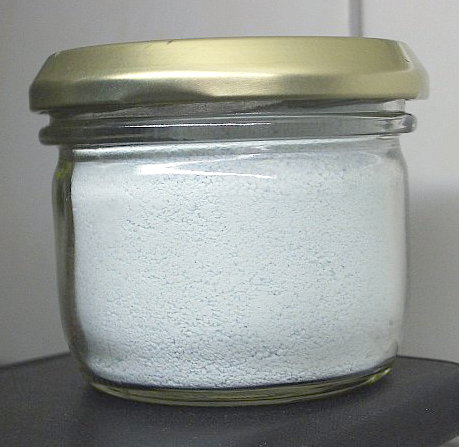
\includegraphics[width=\linewidth,height=4.2cm,keepaspectratio]{images/book1/cuso4-anhydrous.jpg}

{\small Sulfato de cobre anidro: um pó branco. Foto: W.~Oelen,
CC BY-SA 3.0.}
\end{minipage}\hfill
\begin{minipage}[b]{0.48\linewidth}\centering
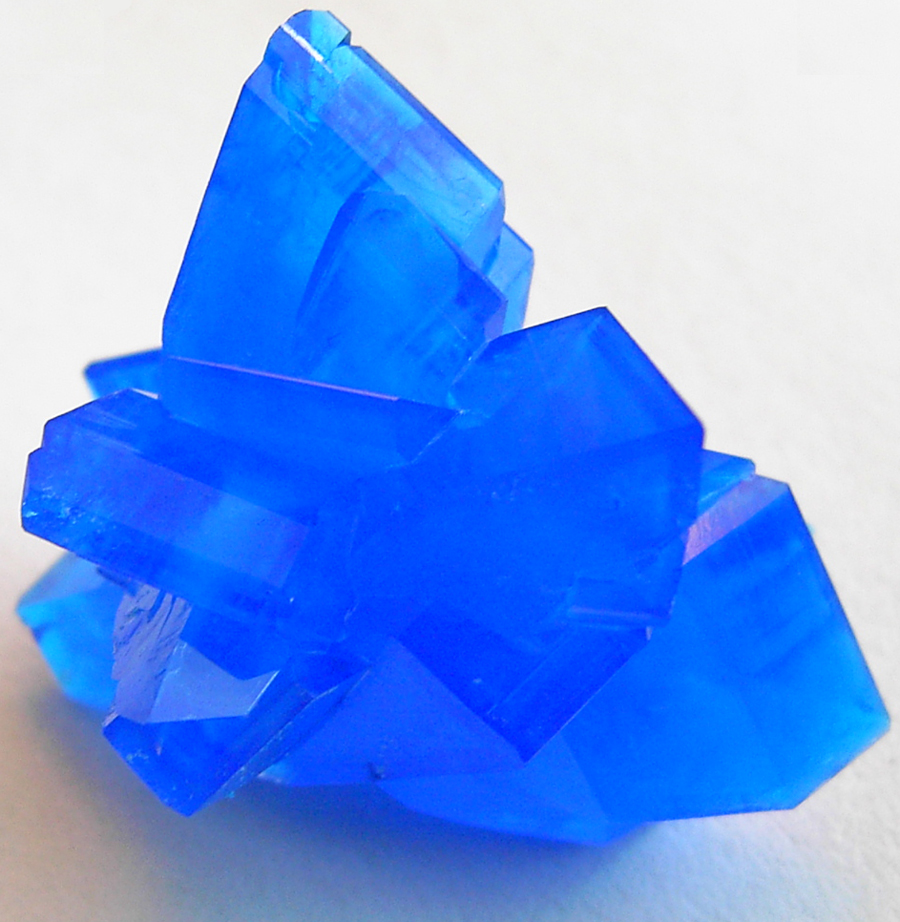
\includegraphics[width=\linewidth,height=4.2cm,keepaspectratio]{images/book1/cuso4-hydrated.jpg}

{\small Com água ele fica azul; estes cristais contêm água. Foto:
Stephanb, CC BY-SA 3.0.}
\end{minipage}
\end{omfigure}

\begin{safety}{\ghs[0.82cm]{GHS05}\ghs[0.82cm]{GHS07}\ghs[0.82cm]{GHS09}}
% ledger: ghs:CuSO4
Sulfato de cobre: nocivo se ingerido e irritante para a pele (GHS07);
pode causar lesões graves nos olhos (GHS05); muito tóxico para os
organismos aquáticos, com efeitos duradouros (GHS09). Óculos de proteção
e luvas; os resíduos são recolhidos, nunca jogados na pia.
\end{safety}

\begin{proposition}[O oxigênio reacende uma tala em brasa]\label{prop:g7:identifying-substances:splint}
Uma tala de madeira é acesa e depois apagada com um sopro, de modo que
só fica uma brasa vermelha. Introduzida num tubo de ensaio com oxigênio,
a tala em brasa volta a pegar fogo.
\end{proposition}

\begin{proposition}[O hidrogênio queima com um estalo agudo]\label{prop:g7:identifying-substances:pop}
Uma tala acesa segurada na boca de um pequeno tubo de ensaio com
hidrogênio produz um ``pop'' curto e agudo: o hidrogênio \omterm{def:g4:what-a-fire-needs:burning}{queima} na hora
com o oxigênio do \omterm{def:g4:air-a-mixture-of-gases:air}{ar}.
\end{proposition}

\begin{omfigure}
\begin{tikzpicture}[font=\small, scale=1.25]
  % splint test for oxygen
  \pic[transform shape] at (0,0) {testtube={0}{white}};
  \draw[brown!60!black, line width=2pt] (0.15,1.6) -- (1.4,3.6);
  \fill[orange!85] (0.15,1.6) circle (0.07);
  \fill[orange!80] (0.12,1.62) .. controls (0.0,1.9) and (0.08,2.1) .. (0.1,2.3)
    .. controls (0.2,2.05) and (0.3,1.85) .. (0.2,1.62);
  \node[anchor=north, align=center] at (0,-0.15) {oxigênio:\\ a tala em brasa\\ volta a pegar fogo};
  % pop test for hydrogen
  \begin{scope}[xshift=4cm]
    \pic[transform shape, rotate=180] at (0,3.1) {testtube={0}{white}};
    \draw[brown!60!black, line width=2pt] (0.05,-0.05) -- (1.3,-0.9);
    \fill[orange!85] (0.05,-0.02) .. controls (-0.05,0.08) and (0.0,0.15) .. (0.02,0.22)
      .. controls (0.08,0.15) and (0.15,0.08) .. (0.1,-0.02);
    \node[font=\small\itshape] at (-0.9,0.15) {pop!};
    \node[anchor=north, align=center] at (0,-1.0) {hidrogênio:\\ um estalo agudo\\ na boca do tubo};
  \end{scope}
\end{tikzpicture}

{\small À esquerda: uma tala em brasa se reacende no oxigênio. À direita:
uma tala acesa na boca de um tubo de hidrogênio virado para baixo dá um
estalo agudo (o hidrogênio é mais leve que o \omterm{def:g4:air-a-mixture-of-gases:air}{ar}, por isso o tubo é
segurado com a boca para baixo).}
\end{omfigure}

\begin{safety}{\ghs[0.82cm]{GHS02}\ghs[0.82cm]{GHS04}}
% ledger: ghs:H2
Hidrogênio: gás extremamente inflamável (GHS02), guardado sob pressão em
cilindros (GHS04). O teste do estalo é feito com poucos mililitros
apenas, pelo professor.
\end{safety}

\section{A cromatografia em papel}

\begin{definition}[Cromatografia em papel e cromatograma]\label{def:g7:identifying-substances:chromatography}
A \emph{cromatografia em papel}\index{cromatografia em papel} separa os
corantes de uma \omterm{def:g6:pure-substances-and-mixtures:mixture}{mistura}. Uma pequena mancha da \omterm{def:g6:pure-substances-and-mixtures:mixture}{mistura} é posta sobre uma
linha traçada perto da base de uma tira de papel; a base da tira
mergulha num \omterm{def:g6:solutions-and-solubility:solute}{solvente}, que sobe devagar pelo papel e leva cada corante
consigo, uns mais depressa que outros. Quando o \omterm{def:g6:solutions-and-solubility:solute}{solvente} subiu quase até
o alto, a tira é retirada e secada: ela é o
\emph{cromatograma}\index{cromatograma}.
\end{definition}

\begin{omfigure}
\begin{tikzpicture}[font=\small, scale=1.3]
  % the strip in a beaker of solvent
  \pic[transform shape] at (0,0) {beaker={0.12}{omWater!80}};
  \fill[white] (-0.42,0.06) rectangle (0.42,2.2);
  \fill[omWater!80] (-0.42,0.06) rectangle (0.42,0.24);
  \draw[omGlass, line width=0.6pt] (-0.42,0.06) rectangle (0.42,2.2);
  \draw[black!60, line width=0.4pt] (-0.42,0.42) -- (0.42,0.42);
  \fill[black!80] (0,0.42) circle (0.07);
  \shade[ball color=black!20] (0,2.27) circle (0.08);
  \draw[black!50, line width=1.2pt] (-1.1,2.27) -- (1.1,2.27);
  \node[anchor=north, align=center] at (0,-0.15) {no início};
  \draw[<-, omProp, thick] (0.1,0.5) -- (1.3,0.8) node[right, text=black]
    {mancha na linha a lápis};
  \draw[<-, omProp, thick] (1.0,2.27) -- (1.3,2.5) node[right, text=black]
    {bastão que segura o papel};
  \draw[<-, omProp, thick] (0.75,0.15) -- (1.3,0.25) node[right, text=black]
    {solvente, abaixo da linha};
  % the chromatogram
  \begin{scope}[xshift=6.2cm]
    \pic[transform shape] at (0,0) {tlcplate};
    \draw[black!50, dashed] (-0.7,2.7) -- (0.7,2.7);
    \fill[blue!70] (0,1.0) ellipse (0.13 and 0.09);
    \fill[red!70] (0,1.7) ellipse (0.13 and 0.09);
    \fill[yellow!80!orange] (0,2.35) ellipse (0.13 and 0.09);
    \node[anchor=north, align=center] at (0,-0.15) {o cromatograma};
    \draw[<-, omProp, thick] (0.75,2.7) -- (1.3,2.85) node[right, text=black]
      {até onde o solvente subiu};
    \draw[<-, omProp, thick] (0.2,1.7) -- (1.3,1.7) node[right, text=black]
      {três corantes: é uma mistura};
  \end{scope}
\end{tikzpicture}

{\small \omterm{def:g7:identifying-substances:chromatography}{Cromatografia em papel} de uma tinta preta. O \omterm{def:g6:solutions-and-solubility:solute}{solvente} sobe pelo
papel e separa a tinta em três corantes.}
\end{omfigure}

\begin{method}[Ler um cromatograma]\label{met:g7:identifying-substances:read}
\begin{enumerate}
  \item Conte as manchas acima de cada ponto de partida: uma mancha, um
        corante; duas manchas ou mais, uma \omterm{def:g6:pure-substances-and-mixtures:mixture}{mistura} de corantes.
  \item Compare as alturas: no mesmo \omterm{def:g7:identifying-substances:chromatography}{cromatograma}, um corante sobe sempre
        até a mesma altura. Uma mancha na mesma altura que um corante
        conhecido provavelmente é esse corante.
  \item Use uma linha a lápis, nunca a tinta: a própria tinta seria
        separada pelo \omterm{def:g6:solutions-and-solubility:solute}{solvente}.
\end{enumerate}
\end{method}

\begin{example}[Os corantes das balas]\label{ex:g7:identifying-substances:sweets}
As coberturas coloridas de algumas balas são raspadas num pouco de água
e aplicadas em manchas numa tira, ao lado de manchas dos corantes
alimentares permitidos em doces. O \omterm{def:g7:identifying-substances:chromatography}{cromatograma} mostra que a cobertura
verde contém um corante amarelo e um corante azul, os dois presentes
entre os corantes permitidos.
\end{example}


\section{Ler uma tabela de testes}

\begin{proposition}[Uma tabela de testes característicos]\label{prop:g7:identifying-substances:bank}
Os químicos reúnem os testes que usam numa tabela, uma tabela de testes,
que se lê da esquerda para a direita:
\begin{center}
\small
\begin{tabular}{llll}
\hline
espécie procurada & \omterm{def:g7:identifying-substances:characteristic-test}{reagente} ou teste & resultado positivo & \\
\hline
dióxido de carbono & água de cal & a água de cal fica leitosa & \\
água & sulfato de cobre anidro & o branco fica azul & \\
oxigênio & tala em brasa & a tala se reacende & \\
hidrogênio & tala acesa & um estalo agudo & \\
corantes de uma \omterm{def:g6:pure-substances-and-mixtures:mixture}{mistura} & \omterm{def:g7:identifying-substances:chromatography}{cromatografia em papel} & uma mancha por corante & \\
\hline
\end{tabular}
\end{center}
\end{proposition}

\begin{remark}[O que um teste não diz]\label{rem:g7:identifying-substances:limits}
Um teste positivo prova que a espécie está presente, não que ela está
sozinha: um líquido que deixa azul o sulfato de cobre contém água, mas
pode ser água salgada ou suco de laranja. Um teste negativo só diz que a
espécie está ausente, ou presente numa quantidade pequena demais para
aparecer.
\end{remark}

\begin{omfigure}
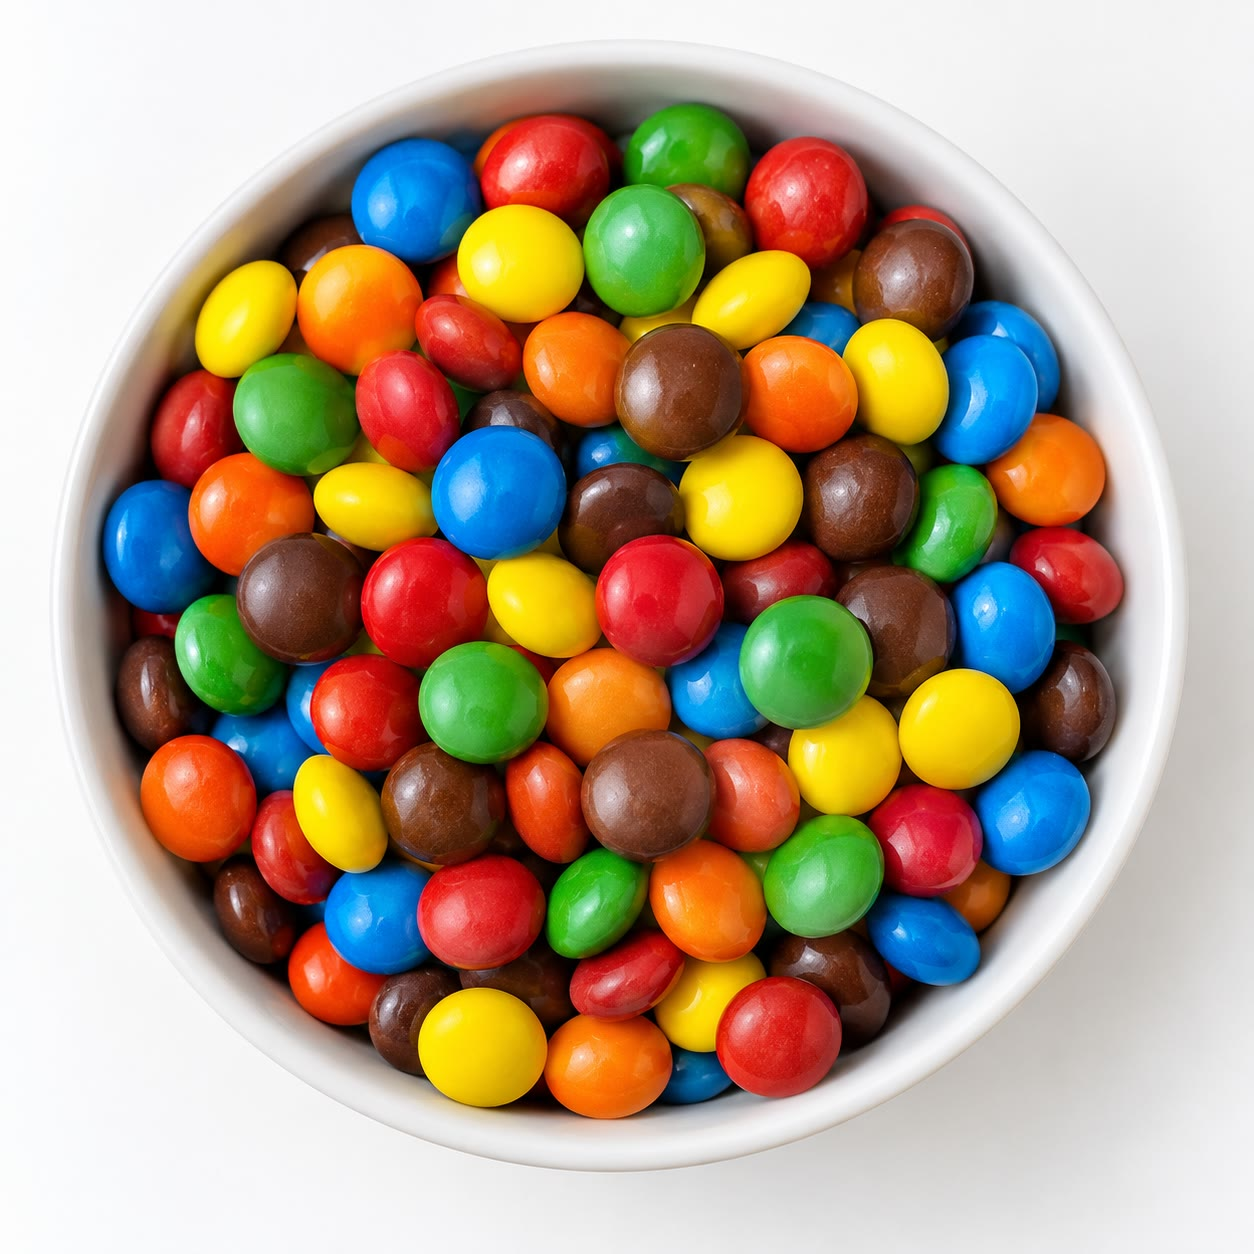
\includegraphics[width=0.32\linewidth]{images/book1/ai/g7-sweets.jpg}

{\small Confeitos coloridos: as cores deles são \omterm{def:g6:pure-substances-and-mixtures:mixture}{misturas} de corantes que
a cromatografia consegue separar.}
\end{omfigure}

\begin{omfigure}
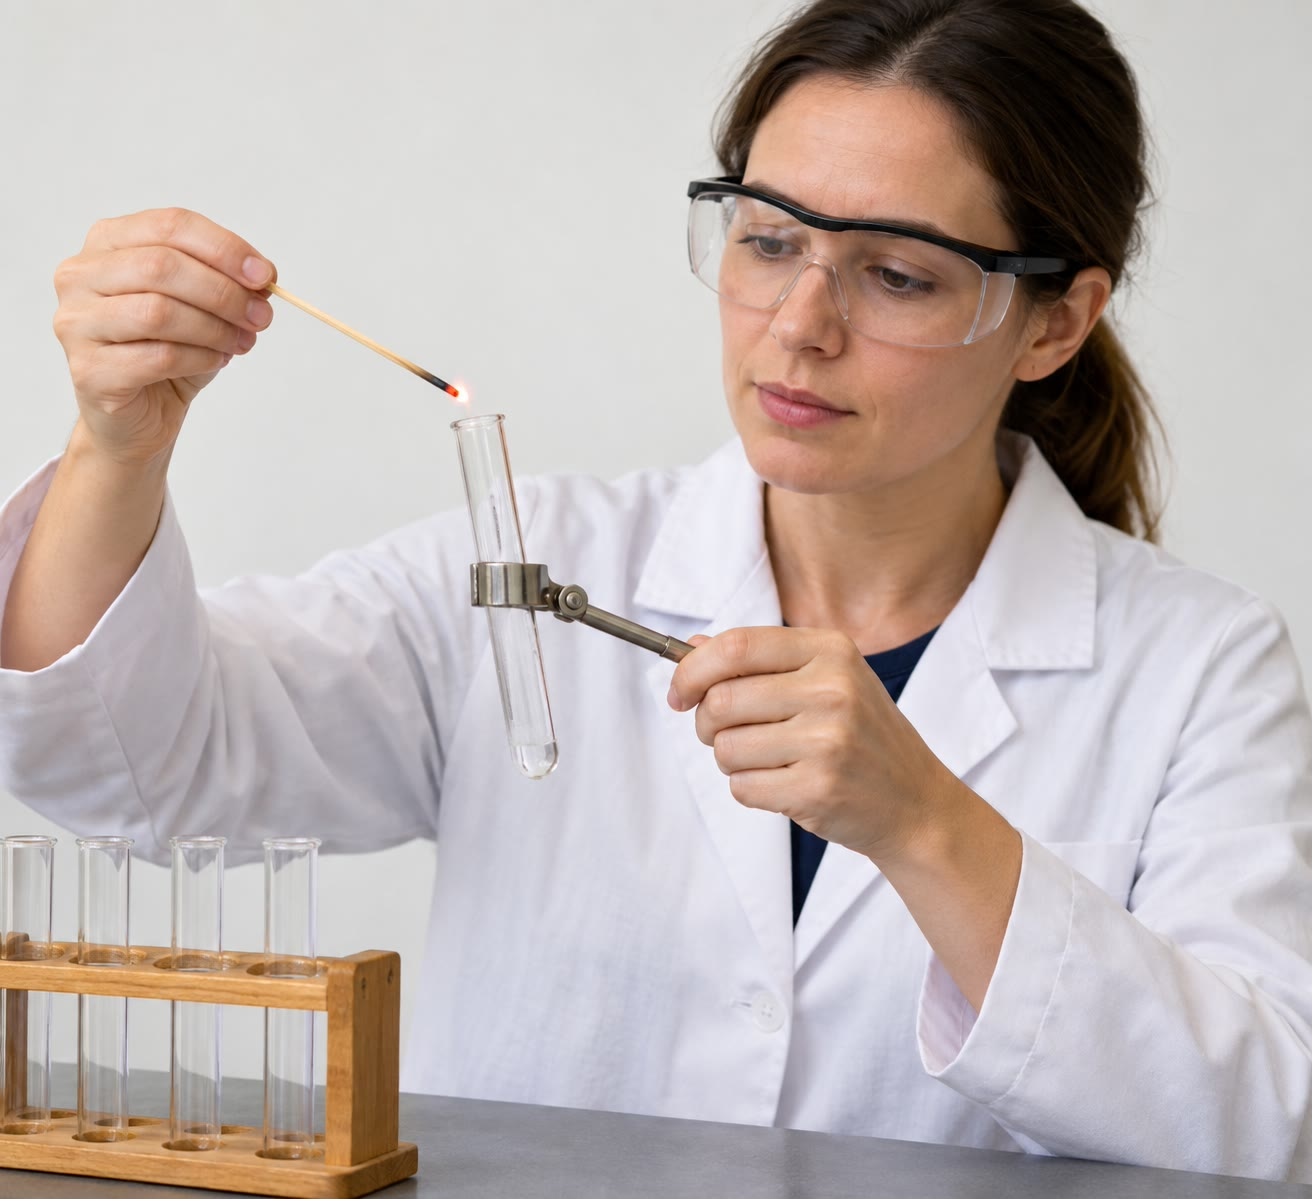
\includegraphics[width=0.36\linewidth]{images/book1/ai/g7-splint-teacher.jpg}

{\small Uma professora testa um gás com uma tala em brasa.}
\end{omfigure}

\section{Exercícios}

\begin{exercise}[$\star$]\label{exo:g7:identifying-substances:1}
Que teste identifica o dióxido de carbono? Descreva o resultado positivo
dele.
\end{exercise}

\begin{exercise}[$\star$]\label{exo:g7:identifying-substances:2}
Um pó branco fica azul quando se pinga um líquido sobre ele. O que isso
mostra sobre o líquido?
\end{exercise}

\begin{exercise}[$\star$]\label{exo:g7:identifying-substances:3}
Uma tala em brasa é introduzida num frasco de gás e volta a pegar fogo.
Que gás o frasco contém?
\end{exercise}

\begin{exercise}[$\star$]\label{exo:g7:identifying-substances:4}
Por que a linha de partida de um \omterm{def:g7:identifying-substances:chromatography}{cromatograma} em papel é traçada a lápis
e não a tinta?
\end{exercise}

\begin{exercise}[$\star\star$]\label{exo:g7:identifying-substances:5}
Por que a linha de partida tem de ficar acima do nível do \omterm{def:g6:solutions-and-solubility:solute}{solvente} no
béquer?
\end{exercise}

\begin{exercise}[$\star\star$]\label{exo:g7:identifying-substances:6}
O \omterm{def:g7:identifying-substances:chromatography}{cromatograma} de uma tinta verde mostra duas manchas, uma na altura de
um corante amarelo de referência, outra na altura de um corante azul de
referência. A tinta verde é uma \omterm{def:g6:pure-substances-and-mixtures:pure-substance}{substância pura}? De que ela é feita?
\end{exercise}

\begin{exercise}[$\star\star$]\label{exo:g7:identifying-substances:7}
Com a tabela de testes, que teste você usaria para mostrar que um gás
liberado por uma reação é o hidrogênio? O que você espera ver?
\end{exercise}

\begin{exercise}[$\star\star$]\label{exo:g7:identifying-substances:8}
O \omterm{def:g4:air-a-mixture-of-gases:air}{ar} expirado turva a água de cal muito mais depressa do que o \omterm{def:g4:air-a-mixture-of-gases:air}{ar}
fresco. O que isso nos diz sobre o \omterm{def:g4:air-a-mixture-of-gases:air}{ar} que expiramos?
\end{exercise}

\begin{exercise}[$\star\star$]\label{exo:g7:identifying-substances:9}
Um líquido límpido deixa azul o sulfato de cobre anidro. O Sam conclui:
``É água pura.'' Explique por que o Sam está errado.
\end{exercise}

\begin{exercise}[$\star\star$]\label{exo:g7:identifying-substances:10}
Olhe o \omterm{def:g7:identifying-substances:chromatography}{cromatograma} da tinta preta neste capítulo. Quantos corantes a
tinta contém? Qual deles subiu mais alto?
\end{exercise}

\begin{exercise}[$\star\star\star$]\label{exo:g7:identifying-substances:11}
Três frascos contêm oxigênio, hidrogênio e dióxido de carbono, mas os
rótulos deles se perderam. Planeje, no papel, os testes que dariam o
nome de cada frasco, numa ordem que use o menor número possível de
testes.
\end{exercise}

\begin{exercise}[$\star\star\star$]\label{exo:g7:identifying-substances:12}
Um aluno testa um gás com água de cal e não vê acontecer nada. Dê duas
explicações possíveis, e o teste de controle que ajudaria a decidir.
\end{exercise}

\section{Problema: o bilhete falsificado}

\begin{problem}[{Problema de fim de semana --- um bilhete escrito com
caneta hidrográfica, três canetas suspeitas, três cilindros de gás sem
rótulo e uma tabela de testes}]
\label{pb:g7:identifying-substances:1}
Pedem ao laboratório de uma escola que ajude a resolver dois pequenos
mistérios. Primeiro, um bilhete escrito com caneta hidrográfica preta
tem de ser associado a uma de três canetas pretas, 1, 2 e 3. Tira-se uma
gota de tinta do bilhete e de cada caneta, e as gotas são aplicadas na
mesma tira de papel, que depois é revelada com água. O \omterm{def:g7:identifying-substances:chromatography}{cromatograma} é
mostrado abaixo.
\begin{center}
\begin{tikzpicture}[font=\small, x=1cm, y=1cm]
  \fill[white] (0,0) rectangle (6,4);
  \draw[omGlass, line width=0.6pt] (0,0) rectangle (6,4);
  \draw[black!60] (0,0.5) -- (6,0.5);
  \draw[black!50, dashed] (0,3.6) -- (6,3.6);
  \foreach \x/\lab in {0.9/bilhete, 2.3/{\shortstack{caneta\\ 1}}, 3.7/{\shortstack{caneta\\ 2}}, 5.1/{\shortstack{caneta\\ 3}}}
    \node[anchor=north] at (\x,-0.05) {\lab};
  % note: three dyes
  \fill[blue!70] (0.9,1.2) ellipse (0.18 and 0.1);
  \fill[red!70] (0.9,2.2) ellipse (0.18 and 0.1);
  \fill[yellow!80!orange] (0.9,3.1) ellipse (0.18 and 0.1);
  % pen 1: two dyes
  \fill[blue!70] (2.3,1.2) ellipse (0.18 and 0.1);
  \fill[black!70] (2.3,2.7) ellipse (0.18 and 0.1);
  % pen 2: same three as the note
  \fill[blue!70] (3.7,1.2) ellipse (0.18 and 0.1);
  \fill[red!70] (3.7,2.2) ellipse (0.18 and 0.1);
  \fill[yellow!80!orange] (3.7,3.1) ellipse (0.18 and 0.1);
  % pen 3: three dyes, other heights
  \fill[violet!70] (5.1,0.9) ellipse (0.18 and 0.1);
  \fill[red!70] (5.1,1.8) ellipse (0.18 and 0.1);
  \fill[green!60!black] (5.1,2.6) ellipse (0.18 and 0.1);
  \node[anchor=west, font=\footnotesize] at (6.1,3.6) {frente do solvente};
  \node[anchor=west, font=\footnotesize] at (6.1,0.5) {linha de partida};
\end{tikzpicture}
\end{center}

\medskip
\noindent\textbf{Parte I --- O \omterm{def:g7:identifying-substances:chromatography}{cromatograma}.}
\begin{enumerate}
  \item Por que as quatro tintas foram aplicadas na mesma tira e
        reveladas juntas?
  \item A tinta do bilhete é uma \omterm{def:g6:pure-substances-and-mixtures:pure-substance}{substância pura} ou uma \omterm{def:g6:pure-substances-and-mixtures:mixture}{mistura}?
        Explique.
  \item Quantos corantes a tinta da caneta 1 contém? A caneta 1 pode ter
        escrito o bilhete?
  \item A caneta 3 também contém três corantes. Por que ela não pode ter
        escrito o bilhete?
  \item Que caneta corresponde ao bilhete? Explique usando as alturas das
        manchas.
\end{enumerate}

\medskip
\noindent\textbf{Parte II --- Três cilindros de gás.}
O segundo mistério: três pequenos cilindros, X, Y e Z, perderam os
rótulos; eles contêm oxigênio, hidrogênio e dióxido de carbono. Um pouco
do gás de cada um é recolhido num tubo de ensaio. O gás X reacende uma
tala em brasa. O gás Y dá um estalo agudo com uma tala acesa. O gás Z
turva a água de cal.
\begin{enumerate}[resume]
  \item Dê o nome do gás X.
  \item Dê o nome do gás Y.
  \item Dê o nome do gás Z.
  \item Antes de testar o gás Z, o aluno borbulha \omterm{def:g4:air-a-mixture-of-gases:air}{ar} comum na mesma água
        de cal durante o mesmo tempo, e ela continua límpida. Como se
        chama esse segundo teste, e o que ele acrescenta à conclusão?
\end{enumerate}

\medskip
\noindent\textbf{Parte III --- A tabela de testes.}
\begin{enumerate}[resume]
  \item Um líquido incolor encontrado ao lado do bilhete deixa azul o
        sulfato de cobre anidro. Escreva a linha da tabela de testes que
        foi usada, e o que o resultado mostra.
  \item Esse resultado prova que o líquido é água pura? Explique.
  \item Conclua o primeiro mistério: quantos corantes a tinta do bilhete
        contém, e que caneta o escreveu?
\end{enumerate}
\end{problem}
